% !TEX program = xelatex
\documentclass[notes=hide]{beamer}
%\documentclass[notes=show]{beamer}
%\documentclass[notes=only]{beamer}
%\documentclass[letterpaper,11pt]{article}
%\usepackage{beamerarticle}

\usepackage{analchem}
\usepackage{lecture}
\sisetup{
	separate-uncertainty=true,
	multi-part-units=single,
	add-decimal-zero=false,
	round-mode=off}
\usepackage{bigdelim}
\usepgfplotslibrary{fillbetween}

\title{Data Processing}
\subtitle{Chapters 3, 4, \& 5}
\author{D.A. McCurry}
\institute{Department of Chemistry and Biochemistry \\ Bloomsburg University}
\date{Fall 2020}

\begin{document}

\maketitle
\mode<article>{\thispagestyle{fancy}}

\frame{\section{Significant Figures}
	\begin{learningobjectives}
		\item Perform calculations to the correct number of significant figures.
		\item Understand why certain digits are significant.
	\end{learningobjectives}
}

\vspace{\stretch{-1}}

\begin{frame}{Where is the error?}
	What is the volume according to the following graduated cylinder?
	\begin{columns}
		\column{2in}
		\begin{center}
		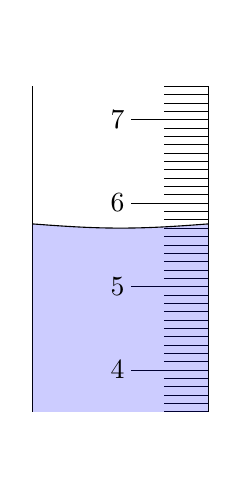
\begin{tikzpicture}
		\begin{axis}[axis x line=none,
			width=1.5in,
			height=2.25in,
			%axis y line=left,
			xmin=0,
			xmax=1,
			ymin=3.5,
			ymax=7.4,
			ytick={3,4,...,8},
			minor y tick num = 9,
			ytick pos = right,
			tick label style = {anchor=east,inner sep=3em},
			major tick length=2.8em,
			minor tick length=1.6em,
			tick style={black},
			y axis line style={-},
			xtick=\empty,
			domain=0:1,]
			\addplot [name path=meniscus,samples=200]
			{-0.05*sin((x+2)*180)+5.75};
			\path[name path=bottom] (axis cs:0,0) -- (axis cs:1,0);
			\addplot[fill=blue,opacity=0.2]
			fill between[
				of=meniscus and bottom,
				];
		\end{axis}
	\end{tikzpicture}
	\end{center}
	\column{0.5\linewidth}
%	\begin{itemize}[<+->]
%		\item Significant figures are used to show in which digit of a
%			number the error lies.
%			\begin{itemize}[<1->]
%				\item It would not make sense to estimate a
%					volume reading of a graduated cylinder
%					with graduations \SI{+-1}{\mL},
%					therefore, error \SI{+-0.1}{\mL} to
%					more than one decimal!
%				\item Nor would it make sense to estimate a
%					volume reading on a buret with
%					graduations \SI{+-0.1}{\mL}, therefore,
%					error \SI{+-0.01}{\mL} to the same one
%					decimal!
%			\end{itemize}
%		\item Tailing and embedded zeros are significant (1\alert{0}6,
%			0.01\alert{0}6\alert{0}, \ldots) but leading zeros are
%			not.
%		\item Scientific notation can help.
%	\end{itemize}
\end{columns}

\end{frame}

\vspace{\stretch{-1}}

\begin{frame}{Rounding}
	\begin{itemize}
		\item Round only the final answer (carry \alert{at least} one
			extra digit throughout the calculations).\footnote{You
			\alert{can} carry all of the extra digits on your
			calculator through to the end.}
		\item When rounding, look at all the digits to be rounded. To 2
			significant figures,
			\begin{center}
				\begin{tabular} {S[table-format=1.9] @{~$=$~} l}
					0.794999999 & \visible<2->{0.79} \\
					0.795000001 & \visible<3->{0.80} \\
					0.795000000 & \visible<4->{0.80}
				\end{tabular}
			\end{center}
	\end{itemize}
\end{frame}

\begin{inclass}
	Add \numlist[list-final-separator={, and }]{1.234e-4;5.67e-6;8.90e-1}:

	\note{\begin{center}
		\begin{tabular} {c S[table-format=1.8]}
		    	  & 0.0001234 \\
			  & 0.00000567 \\
			+ & 0.890 \\ \midrule
			  & 0.89012907 \\
			  & 0.890
		\end{tabular}
	\end{center}
	}

\end{inclass}

\begin{inclass}
	Perform the following calculation:
	\begin{align*}
		\dfrac{\num{1.234e-4} \times \num{8.90e-1}}{\num{5.67e-6}}
	\end{align*}

	\note{\begin{center}
		\begin{tabular} {@{= }S[table-format=2.11]}
			19.369949 \\
			19.4
		\end{tabular}
	\end{center}
	}
\end{inclass}

\frame{\section{Error}
	\begin{learningobjectives}
		\item Recognize the types and causes of experimental error.
		\item Understand the difference between accuracy and precision.
		\item Propagate experimental error through calculations.
	\end{learningobjectives}
}

\vspace{\stretch{-1}}

\begin{frame}[t]{Types of Error}
	\alert{Every} measurement has some uncertainty related to it.

	\only<+>{%
		\begin{block}{Systematic \emph{or} determinate error}
			%\item Systematic \emph{or} determinate error
				\begin{itemize}
					\item Flaws in the system --- equipment or
						experiment design;
						\alert{reproducible}; a bias; can be
						\alert{determined} and eliminated
						\begin{itemize}
							\item pH meter measures low by
								0.1~pH units
							\item buret that is
								\SI{0.05}{\mL} high at
								\SI{30.00}{\mL}
						\end{itemize}
					\item Detecting systematic error:
						\begin{itemize}
							\item Analyze samples of known
								concentration
								%(standard
								%or certified reference
								%materials)
							\item Analyze blanks to make
								sure reagents are not
								``adding'' or hiding
								analyte
							\item Use different methods to measure the analyte
							\item Round robin:  have several individuals or labs perform the analysis on the same sample
						\end{itemize}
				\end{itemize}
			\end{block}
		}

		\mode<article>{\clearpage}

		\only<+>{%
			\begin{block}{Random \emph{or} indeterminate error}
				\begin{itemize}
					\item uncontrolled variables; not reproducible; equal chance of being positive or negative; can be minimized but not eliminated
						\begin{itemize}
							\item electrical noise
							\item parallax
						\end{itemize}
				\end{itemize}
			\end{block}

			\begin{block}{Gross error}
				\begin{itemize}
					\item Major blunders that are generally technician dependent
					\item \alert{Avoid these!}
				\end{itemize}
			\end{block}
		}
\end{frame}

\begin{frame}{Accuracy and Precision}
	\only<+>{%
		\begin{columns}[t]
			\column{0.5\textwidth}
			\begin{block}{Accuracy}
				\begin{itemize}
					\item How close the mean is to the
						``true'' value
					\item Measured by error (absolute error,
						percent error, relative error
				\end{itemize}
			\end{block}
			\column{0.5\textwidth}
			\begin{block}{Precision}
				\begin{itemize}
					\item How well the data from several
						trials holds together
					\item Measured by deviations (standard
						deviation, relative deviation,
						relative standard deviation
				\end{itemize}
			\end{block}
		\end{columns}
	}

	\only<+>{%
		\begin{center}
			\includegraphics[width=\linewidth]{accuracyvprecision.jpg}
		\end{center}
	}
\end{frame}

\begin{frame}[t]{Uncertainty}
	\begin{description}[<+->]
		\item[Absolute uncertainty:] margin of certainty in a
			measurement
			\begin{example}<only@.>
				A class A buret has an uncertainty of
				\SI{+-0.02}{\mL}
					\begin{itemize}[<1->]
						\item \SI{30.23}{\mL} means
							volume between
							\SIrange{30.21}{30.25}{\mL}
						\item \SI{10.12}{\mL} means
							volume between
							\SIrange{10.10}{10.14}{\mL}
					\end{itemize}
			\end{example}
		\item[Relative uncertainty:] the absolute uncertainty
			corrected for size of measurement
			\begin{example}<only@.>
				\begin{align*}
					\frac{0.02}{0.06} &= 0.0006 \text{ or }
						\SI{30.23}{\percent} \\ \\
					\frac{0.02}{10.12} &= 0.002 \text{ or }
						\SI{0.2}{\percent}
				\end{align*}

				\bigskip

				\begin{center}
					\bfseries\usebeamercolor[fg]{alerted text}
					This is a killer for smaller values!
				\end{center}
			\end{example}
	\end{description}
\end{frame}

\begin{frame}{Propagation of Uncertainty}
	For every measurement, error becomes compounded. Consider the following:
	\begin{itemize}
		\item A \SI{10.00(2)}{\mL} pipet is used 4 times to deliver \SI{40.00}{\mL}.
		\item The mass limit on a balance (\SI{\pm0.0005}{\gram}) was \SI{200}{\gram}, so it was used twice for
			a total mass of \SI{350.0000}{\gram}.
	\end{itemize}

	\bigskip

	Where are the sources of error? What are the actual delivered values?
\end{frame}

\begin{frame}[t]{Propagation of Systematic Error}
	\alert{Systematic error} is additive.

	With every transfer, an \alert{uncalibrated} buret \emph{might} be delivering the maximum value within tolerance
	or it might be delivering the minimum.
\end{frame}

\begin{frame}{Tolerances of Class A burets}
	\begin{center}
		\begin{tabular} {@{}S[table-format=3]
			S[table-format=1.2] S[table-format=-1.2]}
			{Buret volume (\si{mL})} & {Smallest graduation
			(\si{\mL})} & {Tolerance (\si{\mL})} \\ \midrule
			5 & 0.01 & +-0.01 \\
			10 & {0.05 \alert{or} 0.02} & +-0.02 \\
			25 & 0.1 & +-0.03 \\
			50 & 0.1 & +-0.05 \\
			100 & 0.2 & +-0.10
		\end{tabular}
	\end{center}
\end{frame}

\begin{frame}{Tolerances of Class A volumetric flasks\footnotemark[2]}
	\begin{center}
%		\scriptsize
		\begin{tabular} {@{}S[table-format=4]
			S[table-format=-1.2]}
			{Flask capacity (\si{\mL})} & {Tolerance (\si{\mL})} \\
			\midrule
			1 & +-0.02 \\
			2 & +-0.02 \\
			5 & +-0.02 \\
			10 & +-0.02 \\
			25 & +-0.03 \\
			50 & +-0.05 \\
			100 & +-0.08 \\
			200 & +-0.10 \\
			250 & +-0.12 \\
			500 & +-0.20 \\
			1000 & +-0.30 \\
			2000 & +-0.50 \\
		\end{tabular}
	\end{center}
	\footnotetext[2]{Class B glassware tolerances are twice
	as large as for Class A}
\end{frame}

\begin{frame}{Tolerances of Class A transfer pipets}
	\begin{center}
%		\scriptsize
		\begin{tabular} {@{}S[table-format=3.1]
			S[table-format=-1.3]}
			{Volume (\si{\mL})} & {Tolerance
			(\si{\mL})} \\ \midrule
			0.5 & +-0.006 \\
			1 & +-0.006 \\
			2 & +-0.006 \\
			3 & +-0.01 \\
			4 & +-0.01 \\
			5 & +-0.01 \\
			10 & +-0.02 \\
			15 & +-0.03 \\
			20 & +-0.03 \\
			25 & +-0.03 \\
			50 & +-0.05 \\
			100 & +-0.08
		\end{tabular}
	\end{center}
\end{frame}
		
\begin{frame}{Manufacturer's tolerances for micropipets}
	\begin{center}
		\scriptsize
		\begin{tabular} {@{}l 
			S[table-format=-1.1] 
			S[table-format=-1.1] 
			S[table-format=-1.1] 
			S[table-format=-1.2] }
			& \multicolumn{2}{c}{\bfseries At
			\SI{10}{\percent} of pipet volume} &
			\multicolumn{2}{c}{\bfseries At
			\SI{100}{\percent}
			of pipet volume} \\
			Pipet volume (\si{\micro\liter}) &
			{Accuracy (\%)} & {Precision
			(\%)} & {Accuracy (\%)} & {Precision
			(\%)} \\ \midrule
			\alert{Adjustable Pipets} \\
			0.2--2 & +-8 & +-4 & +-1.2 & +-0.6 \\
			1--10 & +-2.5 & +-1.2 & +-0.8 & +-0.4 \\
			2.5 -- 25 & +-4.5 & +-1.5 & +-0.08 &
			+-0.2 \\
			10--100 & +-1.8 & +-0.7 & +-0.6 & +-0.15
			\\
			30 -- 300 & +-1.2 & +-0.4 & +-0.4 &
			+-.15 \\
			100 -- 1000 & +-1.6 & +-0.5 & +-0.3 &
			+-0.12 \\ \\
			\alert{Fixed Pipets} \\
			10 & & & +-0.8 & +-0.4 \\
			25 & & & +-0.8 & +-0.3 \\
			100 & & & +-0.5 & +-0.2 \\
			500 & & & +-0.4 & +-0.18 \\
			1000 & & & +-0.3 & +-0.12
		\end{tabular}
	\end{center}
\end{frame}

\vspace{\stretch{-1}}

\begin{frame}{Propagation of Random Error}
	\only<+>{%
		Systematic error can be removed by \emph{calibrating} glassware, but one can \emph{never} remove
		\alert{random error}.

		We can assume that the contribution of random error will be much smaller than that of systematic error.
		We do \alert{not} add random error!
	}

	\only<+>{%
		\begin{center}
			\begin{tabular} {>{$}p{0.4\linewidth}<{$} >{$}p{0.5\linewidth}<{$} }
				\toprule
				\text{\bfseries Function} &
				\text{\bfseries Uncertainty} \\
				\midrule
				y = x_1 + x_2 & e_y = \sqrt{e^2_{x_1} + e^2_{x_2}} \\ \\
				
				y = x_1 - x_2 & e_y = \sqrt{e^2_{x_1} + e^2_{x_2}} \\ \\
	
				y = x_1 \cdot x_2 & \%e_y = \sqrt{\%e^2_{x_1} +
				\%e^2_{x_2}} \\ \\
	
				y = \dfrac{x_1}{x_2} & \%e_y = \sqrt{\%e^2_{x_1} +
				\%e^2_{x_2}} \\
				\bottomrule
				\multicolumn{2}{>{\hangindent=0.1\linewidth}p{0.9\linewidth}}
					{\footnotesize
					$x$ represents a variable and
					$a$ represents a constant that
					has \alert{no}
					uncertainty} \\
				\multicolumn{2}{>{\hangindent=0.1\linewidth}p{0.9\linewidth}}
					{\footnotesize
					$e_x/x$ is the relative error in $x$ and $\%e_x$ is
					$100 \times e_x/x$.}
			\end{tabular}
	\end{center}
}

\only<+>{%
		\begin{center}
			\begin{tabular} {>{$}p{0.4\linewidth}<{$} >{$}p{0.5\linewidth}<{$} }
				\toprule
				\text{\bfseries Function} &
				\text{\bfseries Uncertainty} \\
				\midrule
				y = x^a & \%e_y = a\%e_x \\ \\
				
				y = \log x & e_y = \dfrac{1}{\ln 10} \dfrac{e_x}{x}
				\approx \num{0.43429} \dfrac{e_x}{x} \\ \\
	
				y = \ln x & e_y = \dfrac{e_x}{x} \\ \\
				
				y = 10^x & \dfrac{e_y}{y} = (\ln 10) e_x \approx
				\num{2.3026} e_x \\ \\
	
				y = e^x & \dfrac{e_y}{y} = e_x \\
				\bottomrule
			\end{tabular}
	\end{center}
}

%%	\begin{itemize}
%%		\item To see how all uncertainties affect a calculated value, we
%%			can use standard rules to propagate the uncertainties
%%			throughout a calculation
%%		\item We will use standard deviation or published uncertainty
%%			values (chapter 2)
%%		\item Assume that only random error is present, that systematic
%%			error has been discovered and removed.
%%		\item The summary of rules to propagate error are in Table 3-1
%%			of the text
%%	\end{itemize}
\end{frame}

\begin{frame}[t]{Consider the Synthesis of Au NP Lab}
	For the \SI{1.0}{\milli\Molar} Au sol'n,
		\begin{itemize}
			\item An analytical balance was used with
				tolerance of \SI{+-0.0005}{\gram}
			\item A \SI{100}{\mL} volumetric flask was
				used with a tolerance of \SI{+-0.08}{\mL}
		\end{itemize}

		\begin{enumerate}[<only@+(1)>]
			\item What is the FW of the stock \ch{HAuCl4}?
				\vspace{\stretch{1}}
				\note<2>{%
					\begin{center}
				\begin{tabular} {r l@{ @ }
					S[table-format=3.6(6)]@{ $=$ }S[table-format=3.6(6)]}
					& 7 H & 1.00798(14) & 7.05586(98) \\
					& 1 Au & 196.966569(4) & 196.966569(4) \\
					& 4 Cl & 35.452(7) & 141.808(28) \\
						+ & 3 O & 15.9994(4) & 47.9982(12) \\ \midrule
						\multicolumn{3}{l}{} & 393.828629(28043) \\
						\multicolumn{3}{r}{\bfseries Answer:} & 393.83(3)
				\end{tabular}
					\end{center}
			
				\begin{align*}
					e &= \sqrt{0.00098^2+0.000004^2+0.028^2+0.0012^2} \\
					  &= \num{0.0280042832} = 0.03
				\end{align*}
			}
			
			\item What error is present in the measurement of mass
				and volume?
				\vspace{\stretch{1}}

					\note<3>{
						\SI{0.0396(5)}{\gram} dissolved in \SI{100.00(8)}{\mL} of water.
				\begin{align*}
					[\ch{Au}] &= \frac{\text{g~Au}
					}{(\text{volume \ch{H2O}})(\text{g/mol~\ch{HAuCl4}})} \\
						  &=
						  \frac{\SI{0.0396}{\gram}}{(\SI{0.10000}{\liter})(\SI{393.83}{\gram\per\mole})}
						  = \SI{1.00551}{\milli\Molar}
						  \\
					\%e_{[\ch{Au}]} &= \sqrt{\%e^2_{\text{g~Au}} +
					\%e^2_{\text{volume~\ch{H2O}}}+\%e^2_{\text{g/mol~Au}}} \\
								   &= \sqrt{\left(\frac{0.0005}{0.0396}\times 100\right)^2 +
									   \left(\frac{0.00008}{0.10000}\times
										   100\right)^2 +
										   \left(\frac{0.03}{393.83}\times
									   100\right)^2} \\
								   &= \SI{1.265181056}{\percent} \\
						\therefore \ch{[Au]} &= \boxed{\SI{1.01(1)}{\milli\Molar}}
				\end{align*}
}
\end{enumerate}



	\begin{block}<only@+(1)>{The \alert{REAL} Rule for Significant Figures:}
		The first digit of the absolute uncertainty is the last
		significant digit in the answer.
	\end{block}
\end{frame}

%\note{Determining Mass Error
%
%	\fbox{\SI{0.0393}{\gram} \ch{HAuCl4 * 3 H2O} weighed}
%
%	\vspace{1em}
%
%	\begin{align*}
%			\SI{0.0393 +- 0.0005}{\gram} & \times
%		\dfrac{\SI{1}{\mole}}{\SI{393.83 +- 0.03}{\gram}} \times
%		\dfrac{\SI{1000}{\milli\mole}}{\SI{1}{\mole}} \\
%			&= \SI{0.099789597 +- 0.001269611}{\milli\mole} \\
%		&\approx \SI{0.100 +- 0.001}{\milli\mole}
%	\end{align*}
%
%	For multiplication and division, error is \alert{relative}!
%
%	\begin{align*}
%		\%e_\text{mass} &= \dfrac{0.0030184}{393.83} \times 100 =
%		\SI{0.007664247}{\percent} \\
%		\%e_\text{bal} &= \dfrac{0.0005}{0.0393} \times 100 =
%		\SI{1.272264631}{\percent} \\
%		\%e_\text{tot} &= \sqrt{\%e_\text{mass}^2 + \%e_\text{bal}^2} \\
%		&= \sqrt{(\SI{0.007664247}{\percent})^2 +
%		(\SI{1.272264631}{\percent})^2} \\
%		&= \SI{1.272287716}{\percent} \\
%		e_\text{tot} &= \dfrac{\num{1.272287716}}{100} \times
%		0.099789597 \\
%		&= \num{0.00126961}
%	\end{align*}
%}
%
%\note{The True Concentration
%
%	\begin{align*}
%		\dfrac{\SI{0.100 +- 0.001}{\milli\mole}}{\SI{0.10000 +-
%		0.00008}{\liter}} &= \fbox{\SI{1.00 +- 0.01}{\milli\Molar}}
%	\end{align*}
%
%	\begin{align*}
%		\%e_\text{\# moles} &= \dfrac{0.001\ldots}{0.100\ldots} \times 100 =
%		1.272287716 \\
%		\%e_\text{volume} &= \dfrac{0.00008}{0.10000} \times 100 =
%		0.00008 \\
%		\%e_\text{tot} &= \sqrt{(1.2722877)^2 + (0.00008)^2} \\
%		&= \num{1.272287718} \\
%		e_\text{tot} &= \dfrac{\num{1.2722877}}{100} \times 0.997895966
%		= 0.012696108
%	\end{align*}
%}

\begin{frame}[t]{Every transfer compounds error}
	Assume we prepared \SI{100}{\milli\liter} of solution by pipetting four
	\SI{25.00 +- 0.03}{\milli\liter} aliquots to a vial containing the
	\ch{HAuCl4 * 3 H2O} instead of using a volumetric flask.
	Assume that dissolution of the \ch{HAuCl4 * 3 H2O} did not
	change the volume.

	\begin{alertblock}<+(1)->{Additional error was introduced!}
		A total of 4 transfers requires further propagation of error.
		\begin{equation*}
			e_\text{volume~\ch{H2O}} \neq \SI{+-0.03}{\mL}
		\end{equation*}
	\end{alertblock}

	\note<2>{%
		Instead,
		\begin{enumerate}
			\item $e = 4 \times 0.03 = 0.12 \approx \boxed{0.1}$ for an \emph{uncalibrated} pipet.
			\item Assume that the pipet was calibrated and delivered \SI{24.99(2)}{\mL}:
		\begin{align*}
			V_\text{total} &= V_1 + V_2 + V_3 + V_4 \\
			\therefore e_{V_\text{total}} &= \sqrt{e^2_1 + e^2_2 + e^2_3 +
			e^2_4 } \\
					&= \sqrt{4 \times 0.02^2} = \boxed{\num{0.04}}
		\end{align*}
	\end{enumerate}
	}
\end{frame}

\clearpage

\begin{frame}{Error is relative}
	What happens to our error if we were measuring volumes closer to
	\SIlist[list-final-separator={, or }]{10;1;0.1}{\mL}?

	\bigskip

	\pause

	\begin{block}{Lab Technique Suggestion:}
		It is important to minimize the number of transfers in sample
		preparation as this is a source of \alert{gross error}.
		\begin{itemize}
			\item Use glassware that has been calibrated closer to
				the volume you would like to measure
			\item Use the quantitative transfer technique (remember
				to leave room for rinse volumes!)
			\item Weigh by difference
		\end{itemize}
	\end{block}
\end{frame}

% Ended here on 8-20-2020

\vspace{\stretch{-1}}

\begin{frame}[t]{For Titration Labs}
	Propagate the error in the measurements
		\begin{itemize}
			\item analytical balances are \SI{+-
				0.0005}{\gram}
			\item class A burets are \SI{+-
				0.05}{\milli\liter}
%			\item other burets are \SI{+- 0.1}{\milli\liter}
		\end{itemize}

	How does this value compare with the experimental standard
			deviation?
\end{frame}

\mode<presentation>{%
	\begin{frame}{Consider the Soda Ash lab}
	\begin{enumerate}
		\item mass \ch{Na2CO3} (\SI{+-0.0005}{\gram})
			\begin{align*}
				\underbrace{21.5862}_\text{initial} -
				\underbrace{21.1623}_\text{final} = \SI{0.4239}{\gram}
			\end{align*}
		\item dissolve in water (N/A)
		\item titrate (\SI{+-0.05}{\mL} each unless calibrated)
			\begin{align*}
				\underbrace{38.62}_\text{final} -
				\underbrace{1.15}_\text{initial} =
				\SI{37.47}{\gram}
			\end{align*}
		\item boil (N/A)
		\item continue titration (\SI{+-0.05}{\mL})
			\begin{align*}
				\underbrace{7.66}_\text{final} -
				\underbrace{5.44}_\text{initial} =
				\SI{2.22}{\mL}
			\end{align*}
	\end{enumerate}
	
%	\footnotetext[5]{Some principles will be the same as the Iodometry lab, but
%	this experiment provides a better example for error propagation!}
\end{frame}

\begin{frame}[allowframebreaks]{Order of Operations}
%	Calculate using molar mass from periodic table ($\pm$?~g) to find
%	\si{\Molar}~\ch{HCl}.
%
%	\begin{align*}
%		\dfrac{\SI{0.4239}{\gram}}{\SI{0.03969}{\liter}} \times
%		\dfrac{\SI{1}{\mole}~\ch{Na2CO3}}{\SI{105.9844}{\gram}} \times
%		\dfrac{\SI{2}{\mole}~\ch{HCl}}{\SI{1}{\mole}~\ch{Na2CO3}} =
%		\SI{0.2015}{\Molar}~\ch{HCl}
%	\end{align*}
%
%	But, what is the uncertainty?
%
%	\framebreak

	\begin{itemize}
		\item Uncertainty for addition/subtraction:
			\begin{align*}
				e = \sqrt{e^2_1 + e^2_2 + e^2_3 + \ldots}
			\end{align*}
		\item Uncertainty for multiplication/division:
			\begin{align*}
				\%e = \sqrt{\%e^2_1 + \%e^2_2 + \%e^2_3 +
				\ldots}
			\end{align*}
		\item Mixed calculations will require following the standard
			rules for priority of math operations and multiple
			application of the above.
	\end{itemize}

%	\framebreak
%
%	For molar mass of \ch{Na2CO3},
%	
%	\begin{align*}
%		e &= 2 \times 0.00000002 + 1 \times 0.001 + 3 \times 0.0004 \\
%		  &= 0.00220004 \approx 0.002
%	\end{align*}
%
%	because
%
%	\begin{center}
%		\begin{tabular} {r l@{ @ }S[table-format=2.8]@{ $\pm$
%			}S[table-format=1.8]}
%			& 2 Na & 22.98976928 & 0.00000002 \\
%			& 1 C & 12.0106 & 0.0010 \\
%			+ & 3 O & 15.9994 & 0.0004 \\ \midrule
%			\multicolumn{2}{l}{} & 105.9883386 & 0.00220004
%		\end{tabular}
%	\end{center}
%
%	Thus, $FW_{\ch{Na2CO3}} = \SI{105.988 +- 0.002}{\gram\per\mole}$.
%
%	\framebreak
%
%	\begin{itemize}
%		\item Uncertainty in \ch{Na2CO3} mass:
%			\begin{center}
%				\begin{tabular} {r
%					S[table-format=2.4(4)]}
%					& 21.5862 +- 0.0005 \\
%					- & 21.1623 +- 0.0005 \\ \midrule
%					& 0.4239 +- 0.0007
%				\end{tabular}
%			\end{center}
%		\item Uncertainty is:
%			\begin{align*}
%				e = \sqrt{0.0005^2 + 0.0005^2} &= 0.0007071 \\
%				&\approx 0.0007
%			\end{align*}
%	\end{itemize}
%
%	\framebreak
%
%	\begin{itemize}
%		\item Uncertainty in volumes
%			\begin{center}
%				\begin{tabular} {c
%					S[table-format=2.2]@{ $\pm$
%					}S[table-format=1.2]}
%					& 38.62 & 0.05 \\
%					- & 1.15 & 0.05 \\
%					+ & 7.66 & 0.05 \\
%					- & 5.44 & 0.05 \\ \midrule
%					& 39.69 & 0.1
%				\end{tabular}
%			\end{center}
%		\item Uncertainty is:
%			\begin{align*}
%				e = \sqrt{0.05^2 + 0.05^2 + 0.05^2 + 0.05^2} &=
%				0.1
%			\end{align*}
%	\end{itemize}
%
%	\framebreak
%
%	\begin{itemize}
%		\item Uncertainty in \si{\Molar}~HCl:
%			\begin{center}
%				\begin{tabular} {c
%					S[table-format=3.4]@{ $\pm$
%					}S[table-format=1.4] l}
%					& 0.4239 & 0.0007 & \si{\gram} \\
%					$\times$ & 105.988 & 0.002 &
%					\si{\gram\per\mole} \\
%					$\div$ & 0.3969 & 0.0001 & \si{\liter}
%					\\ \midrule
%					& 0.2015 & 0.0006 & \si{\Molar}
%				\end{tabular}
%			\end{center}
%		\item Uncertainty is:
%			\begin{align*}
%				\%e &= \sqrt{
%				\begin{multlined}
%					\bigg(\dfrac{0.0007}{0.4239} \times
%					100\bigg)^2 +
%					\bigg(\dfrac{0.002}{105.988} \times
%					100\bigg)^2 \\
%					+ \bigg(\dfrac{0.0001}{0.03969} \times
%					100 \bigg)^2 
%				\end{multlined}} \\ &=
%				\sqrt{0.0908} = 0.301\% \\
%				& \dfrac{0.301}{100} \times 0.2015 = 0.0006
%			\end{align*}
%	\end{itemize}
\end{frame}
}

\begin{frame}[t]{Propagating Error in pH}
	Let's consider a \SI{0.2015(6)}{\Molar}~\ch{HCl} solution.
	What is the \pH?

	\note{%
		Recall:
		\begin{align*}
			\text{pH} &= -\log [\ch{H3O+}] \\
			\shortintertext{HCl is a strong acid, thus we assume}
			[\ch{H3O+}] &= \SI{0.2015}{\Molar} \\
			\therefore \text{pH} &= -\log(0.2015) = 0.69572495
			\shortintertext{For error:}
			e_y &= \dfrac{1}{\ln 10} \dfrac{e_x}{x} \approx 0.43429
			\dfrac{e_x}{x} \\
			&\approx 0.43429 \times \dfrac{0.0006}{0.2015} \approx 0.001 \\
			\text{Thus,~} \pH &= \num{0.696 +- 0.001}
		\end{align*}
	}
\end{frame}

\clearpage

\frame{\section{Statistics}
	\begin{learningobjectives}
		\item Understand the Gaussian distribution.
		\item Explain the source of certainty of your measurements.
		\item Determine experimental uncertainty from repeated
			measurements.
	\end{learningobjectives}
}

{
	\usebackgroundtemplate{\includegraphics[height=\paperheight]{redbloodcells.jpg}}
	\begin{frame}
		\begin{exampleblock}{Harris, pg. 64}
			so it is never possible to be completely certain of a result.
			Nevertheless, we often seek the answers to questions such as
			``Is my red blood count today higher than usual?'' If today's
			count is twice as high as usual, it is probably truly higher
			than normal. But, what if the ``high'' count is not excessively
			above ``normal'' counts?
		\end{exampleblock}
	\end{frame}
}

\begin{frame}{All measurements contain experimental error}
		\begin{center}
			\begin{tabular} {S l l}
				\multicolumn{2}{l}{\bfseries Count on ``normal'' days} & {\bfseries Today's count} \\ \midrule
				5.1 & \rdelim\}{5}{1ex}[$\times$ \SI{e6}{cells\per\micro\liter}] & \\
				5.3 & & \\
				4.8 & & {\usebeamercolor[fg]{alerted
				text}\bfseries\SI{5.6e6}{cells\per\micro\liter}} \\
				5.4 \\
				5.2 \\
				\multicolumn{2}{l}{Average =
				\SI{5.16e6}{cells\per\micro\liter}}
			\end{tabular}
		\end{center}
	
		\begin{itemize}
			\item How high is too high?
			\item What defines ``normal'' limits?
		\end{itemize}
\end{frame}

\begin{frame}{Effect of 4 small, random errors}
	\centering
	\begin{tikzpicture}
		\node(datas) {
		\scriptsize
		\begin{tabularx}{0.6\linewidth} {c c c c X r }
			I & I & I & I & \centering 1 case all positive & +4u \\
			\\
			D & I & I & I &
			\rdelim\}{4}{1ex}[\parbox{18ex}{\sffamily \centering 4 cases with 3
			positive and 1 negative}] & \multirow{4}{*}{+2u} \\
			I & D & I & I \\
			I & I & D & I \\
			I & I & I & D \\ \\
			D & D & I & I & 
			\rdelim\}{6}{1ex}[\parbox{18ex}{\sffamily \centering 6 cases with 2
			positive and 2 negative}] & \multirow{6}{*}{+0u} \\
			D & I & D & I \\
			D & I & I & D \\
			I & D & D & I \\
			I & D & I & D \\
			I & I & D & D \\ \\
			D & D & D & I &
			\rdelim\}{4}{1ex}[\parbox{18ex}{\sffamily \centering 4 cases with 1
			positive and 3 negative}] & \multirow{4}{*}{-2u} \\
			D & D & I & D \\
			D & I & D & D \\
			I & D & D & D \\ \\
			D & D & D & D & \centering 1 case all negative & -4u
		\end{tabularx}};
	\node[anchor=west] at (datas.east) {
		\includegraphics[width=0.4\linewidth]{small-distro.png}};
	\end{tikzpicture}
\end{frame}

\begin{frame}{Effect of thousands of random errors}
	\begin{columns}
		\column{0.6\linewidth}
		\begin{block}{Gaussian Distribution}
			Results tend to cluster symmetrically around the average
			value when only random error is considered.
		\end{block}

		The width of the Gaussian peak is the standard deviation:
		\begin{center}
		\begin{tabular} {@{$\pm$}l@{$\sigma$ covers }r@{\%
			of peak width}}
			1 & 63.8 \\
			2 & 95.5 \\
			3 & 99.7
		\end{tabular}
		\end{center}
		\column{0.4\linewidth}
		\includegraphics[scale=0.4]{gaussian.png}
	\end{columns}
\end{frame}

\begin{frame}{Means and Standard Deviation}
	\only<+>{%
	\begin{columns}
		\column{0.5\linewidth}
		\begin{itemize}
			\item experimental, $\bar{x}$ and $s$
				\begin{itemize}
					\item values for a small data set
					
					\item \texttt{=STDEV()} in ``Excellian''
					\item $n-1$ = \alert{degrees of freedom}
				\end{itemize}
		\end{itemize}
		\column{0.5\linewidth}
			\begin{align*}
				\bar{x} &= \dfrac{\sum_i x_i}{n}
				\\
				s &= \sqrt{\dfrac{\sum_i
				(x_i - \bar{x})^2}{n-1}}
			\end{align*}
	\end{columns}

	\begin{columns}
		\column{0.5\linewidth}
		\begin{itemize}
			\item population, $\mu$ and $\sigma$
				\begin{itemize}
					\item values for a large (infinite) data
						set
					\item $\mu$ is the \alert{population}
						mean
					\item \texttt{=STDEVP()} in
						``Excellian''
				\end{itemize}
		\end{itemize}
		\column{0.5\linewidth}
			\begin{align*}
				\sigma =
				\sqrt{\dfrac{\sum_i (x_i
				- \bar{x})^2}{n}}
			\end{align*}
	\end{columns}

	\begin{columns}
		\column{0.9\linewidth}
	\begin{itemize}
		\item What about significant figures?
	\end{itemize}
		\column{0.1\linewidth}
	\end{columns}
}	

\only<+>{%
	\begin{block}{Relative Standard Deviation}
		Standard deviation as expressed normalized for mean value.
	\end{block}

	\begin{itemize}
		\item Maintain SFs of $s$!
			\begin{align*}
				\text{RSD} = \dfrac{s}{\bar{x}} & \\
				&\times 100 \text{ is percent RSD} \\
				&\times 1000 \text{ is ppth RSD}
			\end{align*}
		\item Why RSD?
			\begin{itemize}
				\item Credits precision with magnitude of stuff:
					\begin{align*}
						\dfrac{0.012}{12.00} = \SI{1}{ppth}
						\qquad
						\dfrac{0.12}{24.00} = \SI{0.5}{ppth} \leftarrow{} \text{oops!}
					\end{align*}
			\end{itemize}
		\item What about SFs?
	\end{itemize}
}
\end{frame}

\begin{frame}[t]{Standard Deviation of the Mean}
	The more times you perform an experiment, the more certain you are that
	the mean is close to the population mean.
	\begin{align*}
		\sigma_n = \dfrac{\sigma}{\sqrt{n}}
	\end{align*}

%	\pause
%
%	\mode<presentation>{\bigskip}
%	
%	\begin{block}{Experiment 4: Turbidimetric Determination of Sulfate}
%		What is the sulfate concentration between Dead Cow Mine and
%		Hank's Coal Reserve runoff? How does this concentration differ
%		between each of your replicates? How does your determined
%		average compare with the class?
%	\end{block}
\end{frame}

\vspace{\stretch{-0.25}}

\frame{\section{Comparison of Means}
	\begin{learningobjectives}
		\item Know how to compare results with a ``known'' or previously
			obtained value(s).
		\item Read $F$ and $t$ tables for a particular confidence interval.
		\item Explain if a result significantly differs from another.
		\item Be able to identify and eliminate outliers.
	\end{learningobjectives}
}

\vspace{\stretch{-1}}

\begin{frame}{Comparing Standard Deviations}
\only<+>{%
	\begin{itemize}
		\item The \alert{$F$ test} is used to decide whether two
			standard deviations are \alert{significantly different}
			from each other.
			\begin{align*}
				F_\text{calculated} = \dfrac{
					\tikz[baseline,remember picture]{ \node
					[anchor=base, inner sep=0pt]
					(num) {$s_1^2$}; }}{s_2^2}
			\end{align*}
			\begin{tikzpicture}[overlay,remember picture]
				\draw[thick,black,<-,shorten <= 1ex] (num.east) -- ++(0.5,0) node[right, text = black] {\scriptsize larger $s$ in numerator!};
			\end{tikzpicture}
		\item If $F_\text{calculated} > F_\text{table}$, then the two
			data sets have less than a 5\% chance of coming from
			distributions with the same population standard
			deviation.
	\end{itemize}
}

\only<+>{%
	\includegraphics[width=\linewidth]{Ftable.png}
}

	\mode<article>{\clearpage}

\only<+>{%
	\includegraphics[width=\linewidth]{table4-2.png}

	\vspace{2em}

	Is the standard deviation from the substitute instrument significantly
	greater than that of the original instrument?

\note{
	\begin{align*}
		F_{\text{calculated}} &= \dfrac{s_1^2}{s_2^2} \\
		&= \dfrac{(0.47)^2}{(0.28)^2} \\
		&= 2.8_2
	\end{align*}

	From Table 4-3, for 3 degrees of freedom for $s_1$ and 9 degrees of
	freedom for $s_2$, $F_{\text{calculated}} < F_{\text{table}}$, so we
	\alert{reject} the hypothesis that $s_1$ is significantly larger than
	$s_2$.

	\textbf{Note what happens if number of measurements increases!}
	}
}
\end{frame}

\begin{frame}{Confidence Intervals}
	\only<+>{%
	\begin{itemize}
		\item One statistical tool we have is the confidence interval or
			the range of data that we think the true mean would be
			in assuming only random error.
		\item It revolves around a statistical value called Student’s t
			\begin{itemize}
				\item W.S. Gosset of the Guinness Brewery was
					able to publish only under a pseudonym
					of ``Student''
			\end{itemize}
	\end{itemize}

	\begin{block}{Student's t}
	\begin{columns}
	\column{0.5\linewidth}
	\begin{align*}
		\mu = \bar{x} \pm \dfrac{ts}{\sqrt{n}}
	\end{align*}
		\column{0.5\linewidth}
		$t$ is the student

		$s$ is the standard deviation

		$\bar{x}$ is the mean

		$n$ is the number of trials
	\end{columns}
	\end{block}
	}

	\only<+>{%
		\includegraphics[width=\linewidth]{ttable.png}
	}
\end{frame}

\mode<presentation>{
	\begin{frame}{William Sealy Gosset}{Head Brewer of Guinness}
		\begin{columns}
			\column{0.4\linewidth}
			\includegraphics[width=\linewidth]{William_Sealy_Gosset.jpg}
			\column{0.6\linewidth}
			\begin{quote}
				\raggedright
				At Guinness the scientific brewers, including
				Gosset, were allowed by the company to publish
				research so long as they did not mention (1)
				beer, (2) Guinness, or (3) their own
				surname.\footnotemark
			\end{quote}
		\end{columns}

		\footnotetext{Ziliak, S.T. \textit{The American
		Statistician}, \textbf{2019}, 73:sup1, 281-290.}
	\end{frame}
}

\begin{frame}{Confidence Interval Example}
	\only<+>{%
	Let's find \SIlist{50;95;99}{\percent} CIs:
	
	\begin{center}
		\begin{tabular} {@{}S l l}
			\multicolumn{2}{l}{\bfseries Count on ``normal'' days} &
			{\bfseries Today's count} \\ \toprule
			5.1 & \rdelim\}{5}{1ex}[$\times$
			\SI{e6}{cells\per\micro\liter}] & \\
			5.3 & & \\
			4.8 & & \SI{5.6e6}{cells\per\micro\liter} \\
			5.4 \\
			5.2 \\ \bottomrule
		\end{tabular}
	\end{center}
	\begin{columns}
		\column{0.5\linewidth}
		\begin{align*}
			\mu &= \bar{x} \pm \dfrac{ts}{\sqrt{n}}
			= \bar{x} \pm tu_x \\
			\shortintertext{where}
			u_x &=
			\underbrace{\tfrac{s}{\sqrt{n}}}_{\mathclap{\text{standard
			uncertainty}}}
		\end{align*}
		\column{0.5\linewidth}
	\begin{align*}
		\bar{x} &= \num{5.16e6} \\
		s &= \num{0.23e6} \\
		t &= \underbrace{\underbrace{0.741}_{50\%}, \underbrace{2.776}_{95\%},
		\underbrace{4.606}_{99\%}}_{\text{4 degrees of freedom}}
	\end{align*}
	\end{columns}
}

\only<+>{%
	\begin{center}
		\sisetup{table-format=1.2e1}
		\begin{tabular} {r@{\% CI:\qquad}S@{ $\leq \mu \leq$ } S}
		50 & 5.07e6 & 5.25e6 \\
		95 & 4.84e6 & 5.48e6 \\
		99 & 4.63e6 & 5.69e6
	\end{tabular}
	\end{center}

	\begin{itemize}
		\item The more confidence we want, the larger the range of data
			must be!
		\item 50\% indicates the chance is 1 in 2 that the true mean is
			inside the stated range (and 1 in 2 that it is not!)
		\item 95\% indicates the chance is 19 in 20 that the true mean is
			inside the range
		\item \SI{5.6e6}{cells\per\micro\liter} \alert{looks} high since
			it fits only at 99\% and up!
	\end{itemize}
}
\end{frame}

\begin{frame}{Utility of confidence intervals}
	\begin{columns}
		\column{0.5\linewidth}
	\begin{itemize}
		\item The Confidence Interval is a simple useful test but it can
			not do anything more than \alert{predict} where the true
			mean is expected to lie given experimental values and
			statistical constraints!
		\item It is used to design quality assurance charts (control
			charts) for manufacturing plants (chapter 5).
	\end{itemize}
		\column{0.5\linewidth}
		\includegraphics[scale=0.4]{CIchart.png}
	\end{columns}
\end{frame}

\begin{frame}{Comparison of two means}
	{i.e., ``Is our percent error \alert{too} high?''}

	\begin{description}[<+->]
		\item[Case 1:] Comparing to a ``known'' value
		        \begin{itemize}[<1->]
		        	\item Measure the sample multiple times and
		        		compare to the accepted value using $t$.
		        \end{itemize}
		\item[Case 2:] Comparing replicate measurements
		        \begin{itemize}[<1->]
		        	\item Measure 2 samples by 1 technique or 1
		        		sample by 2 techniques and compare
		        		values.
		        \end{itemize}
		\item[Case 3:] Comparing individual differences
			\begin{itemize}[<1->]
				\item Measure multiple samples by 2 techniques
					or 2 samples by multiple techniques.
			\end{itemize}
	\end{description}
\end{frame}

\begin{frame}{Case 1: Comparing a measured result with a ``known'' value}
	\begin{itemize}
		\item Replication of \alert{one} sample using \alert{one}
			technique
			\begin{align*}
				\text{CI} &= \bar{x} \pm \dfrac{ts}{\sqrt{n}}
			\end{align*}
		\item If the measured $x$ is outside of the CI, there is less
			than a 5\% chance (assuming 95\% CI) that the technique or sample agrees
			with the known $x$.
	\end{itemize}

	\begin{block}{Rearranging CI for easier $t$ comparison}
		\begin{columns}
			\column{0.4\linewidth}
			\begin{align*}
				t_{\text{calculated}} &= \dfrac{|x -
				\bar{x}|}{s} \times \sqrt{n}
			\end{align*}
			\column{0.4\linewidth}
			If $t_{\text{calculated}} > t_{\text{table}}$, the
			measured $x$ is \alert{outside} of the
			\alert{selected} CI.
		\end{columns}
	\end{block}
\end{frame}

\begin{frame}[t]{Case 1: Example (Problem 4-22)}
		A SRM is certified to contain 94.6 ppm of an organic
		contaminant.  Your analysis yields: 98.6, 98.4, 97.2,
		94.6, and 96.2 ppm.  Do your results differ at the
		95\% level?


% Ended here on 2020-08-25, did not solve the problem

			\note<+>{%
				\begin{columns}
					\column{0.3\linewidth}
					\begin{tabular} {r@{ = }l}
						mean & $97.0_0$ \\
						std dev & $1.6_6$ \\
						t (95\%, 4 DF) & $2.776$
					\end{tabular}
					\column{0.4\linewidth}
					\begin{align*}
						t_{\text{calculated}} &=
						\dfrac{|x - \bar{x}|}{s} \times
						\sqrt{n} \\
						&= \dfrac{|94.6 - 97.0|}{1.6_6} 
						\times \sqrt{5} \\
						&= 3.24
					\end{align*}
				\end{columns}
				
				\bigskip

				Since $3.24 > 2.776$, the results \alert{do
				differ} at the 95\% CI.
			
				}
	\begin{itemize}[<+->]
		\item What would your conclusion be if one more trial of 94.5
			is done?
			\note<.>{%
				\begin{columns}
					\column{0.3\linewidth}
					\begin{tabular} {r@{ = }l}
						mean & $96.5_8$ \\
						std dev & $1.8_0$ \\
						t (95\%, 5 DF) & $2.571$
					\end{tabular}
					\column{0.4\linewidth}
					\begin{align*}
						t_{\text{calculated}} &=
						\dfrac{|x - \bar{x}|}{s} \times
						\sqrt{n} \\
						&= \dfrac{|94.6 - 96.5_8|}{1.8_0} 
						\times \sqrt{6} \\
						&= 2.702
					\end{align*}
				\end{columns}
				
				\bigskip

				Since $2.70 > 2.571$, the results \alert{still
				differ} at the 95\% CI.
			
				}
	\end{itemize}
\end{frame}

\begin{frame}{Case 2: Comparing replicate measurements}
	\only<+>{%
		\begin{itemize}
		\item Comparing two \alert{sets} of data to determine if they
			agree \alert{within experimental error}
		\item Procedure:
			\begin{enumerate}
				\item Perform $F$ test
				\item Perform $t$ test
			\end{enumerate}
	\end{itemize}

	\begin{block}{If \alert{not} significantly different,}
	\begin{align*}
		t_{\text{calculated}} &= \dfrac{|\bar{x}_1 -
		\bar{x}_2|}{s_{\text{pooled}}} \sqrt{\dfrac{n_1n_2}{n_1+n_2}} \\
		\shortintertext{where}
		\tikz[baseline,remember picture]{\node(spool)
		{$s_{\text{pooled}}$};} &= \sqrt{\dfrac{\sum_{\text{set 1}}
		(x_i - \bar{x}_1)^2 + \sum_{\text{set 2}}
		(x_i - \bar{x}_2)^2}{n_1+n_2 - 2}}
	\end{align*}
		\begin{tikzpicture}[overlay,remember picture]
			\draw[<-,thick] (spool.south) to [in=180,out=270]
			++(0.7,-1) node[right] {\scriptsize weighted average of
			standard deviations.};
		\end{tikzpicture} 
	\end{block}
}

\only<+>{%
	
	\begin{block}{If significantly different,}
		\begin{align*}
			t_{\text{calculated}} &= \dfrac{|\bar{x}_1 -
			\bar{x}_2|}{\sqrt{(s^2_1/n_1) + (s^2_2/n_2)}} \\
			\text{Degrees of freedom} &= \dfrac{(s^2_1/n_1 +
			s^2_2/n_2)^2}{\dfrac{(s^2_1/n_1)^2}{n_1 - 1} +
			\dfrac{(s^2_2/n_2)^2}{n_2 - 1}}
		\end{align*}
	\end{block}

	\begin{itemize}
		\item Why?
			\begin{itemize}
				\item If the deviations are significant enough,
					they may skew the calculation of $t$
			\end{itemize}
		\item What is $\dfrac{s^2}{n}$?
	\end{itemize}
}

\only<+>{%
	\begin{itemize}
		\item What does this test literally mean?
	\end{itemize}

	\begin{center}
		\includegraphics[width=\linewidth]{literalt.jpg}
	\end{center}

}

\only<+>{%

	\begin{center}
		\begin{tikzpicture}[scale=0.7]
			\tikzset{caption/.style={below,font=\small}};
			\tikzset{between/.style={midway,text width=0.2\linewidth, align=center}};
			\node(calcgtab) {\includegraphics[scale=0.2]{bigtcalc.jpg}};
			\node[caption] at (calcgtab.south) {$t_{\text{calc}} > t_{\text{table}}$};
			\node[right = 0.3\linewidth of calcgtab](calcatab) {\includegraphics[scale=0.2]{sametcalc.jpg}};
			\node[caption] at (calcatab.south) {$t_{\text{calc}} \approx t_{\text{table}}$};
			\node[below = of calcgtab](calcltab1) {\includegraphics[scale=0.2]{smalltcalc.jpg}};
			\node[caption] at (calcltab1.south) {$t_{\text{calc}} < t_{\text{table}}$};
			\node[below = of calcatab](calcltab2) {\includegraphics[scale=0.2]{smalltcalc2.jpg}};
			\node[caption] at (calcltab2.south) {$t_{\text{calc}} < t_{\text{table}}$};
			\path (calcgtab) to node[between] {$\Delta$ average makes a difference}	(calcatab);
			\path (calcltab1) to node[between] {So does $\Delta$ width!}(calcltab2);
		\end{tikzpicture}
	\end{center}
}
\end{frame}

\begin{frame}[t]{Case 2: Example (Problem 4-23)}
	\only<+>{%
	Nitrite (\ch{NO2-}) was measured by two methods in rainwater and
	unchlorinated drinking water.  The results ($x \pm s$ ($n$)) are:
	\begin{center}
		\sisetup{table-format=1.3(3),separate-uncertainty}
		\small
		\begin{tabular} {l S l@{\quad}S l}
			{Sample source} & \multicolumn{2}{l}{GC (ppm)} &
			\multicolumn{2}{l}{UV-Vis (ppm)} \\
			\midrule
			rainwater & 0.069(5) & $(n=7)$ & 0.063(8) & $(n=5)$ \\
			drinking water & 0.078(7) & $(n=5)$ & 0.087(8) & $(n=5)$
		\end{tabular}
	\end{center}

	\begin{enumerate}
		\item Do the methods agree (95\%) for both types of water?
		\item For each method, does drinking water contain more nitrite
			(again at 95\%)?
	\end{enumerate}
}

\only<+>{%
	\begin{center}
		\sisetup{table-format=1.3(3),separate-uncertainty}
		\small
		\begin{tabular} {l S l@{\quad}S l}
			{Sample source} & \multicolumn{2}{l}{GC (ppm)} &
			\multicolumn{2}{l}{UV-Vis (ppm)} \\
			\midrule
			\color{blue} rainwater & \color{blue} 0.069(5) & \color{blue} $(n=7)$ &
			\color{blue} 0.063(8) & \color{blue} $(n=5)$ \\
			drinking water & 0.078(7) & $(n=5)$ & 0.087(8) & $(n=5)$
		\end{tabular}
	\end{center}

	\note{
		\begin{align*}
		F &= 2._{56} < F_{\text{table}} (4.53) \\
		t_{\text{calc}} &= \dfrac{|\bar{x}_1 -
		\bar{x}_2|}{s_{\text{pooled}}} \sqrt{\dfrac{n_1n_2}{n_1+n_2}} =
		1.03 \\
		s_{\text{pooled}} &= \sqrt{\dfrac{s_1^2(n_1-1) + s_2^2(n_2-1)}
		{n_1+n_2 - 2}} = 0.006_4\\
		t_{\text{table}} (\text{95\%, 10 DF}) &= 2.228
	\end{align*}

	\begin{center}
	\fbox{Since $t_{\text{calc}} < t_{\text{table}}$, the means are
	statistically identical at 95\%.}
	\end{center}
}}

\mode<article>{\vspace{\stretch{4}}
\clearpage}

\only<+>{%
	\begin{center}
		\sisetup{table-format=1.3(3),separate-uncertainty}
		\small
		\begin{tabular} {l S l@{\quad}S l}
			{Sample source} & \multicolumn{2}{l}{GC (ppm)} &
			\multicolumn{2}{l}{UV-Vis (ppm)} \\
			\midrule
			rainwater & 0.069(5) & $(n=7)$ &
			0.063(8) & $(n=5)$ \\
			\color{blue} drinking water & \color{blue} 0.078(7) & \color{blue} $(n=5)$ & \color{blue} 0.087(8) & \color{blue} $(n=5)$
		\end{tabular}
	\end{center}

	\note{%
	\begin{align*}
		F &= 1._{31} < F_{\text{table}} (4.53) \\
		t_{\text{calc}} &= \dfrac{|\bar{x}_1 -
		\bar{x}_2|}{s_{\text{pooled}}} \sqrt{\dfrac{n_1n_2}{n_1+n_2}} =
		1.90 \\
		s_{\text{pooled}} &= \sqrt{\dfrac{s_1^2(n_1-1) + s_2^2(n_2-1)}
		{n_1+n_2 - 2}} = 0.007_5\\
		t_{\text{table}} (\text{95\%, 8 DF}) &= 2.306
	\end{align*}

	\begin{center}
	\fbox{Since $t_{\text{calc}} < t_{\text{table}}$, the means are
	statistically identical at 95\%.}
	\end{center}
}}

\mode<article>{\vspace{\stretch{1}}}

\only<+>{%
	\begin{center}
		\sisetup{table-format=1.3(3),separate-uncertainty}
		\small
		\begin{tabular} {l >{\color{blue}}S
			>{\color{blue}}l@{\quad}S l}
			{Sample source} & \multicolumn{2}{l}{\color{blue} GC (ppm)} &
			\multicolumn{2}{l}{UV-Vis (ppm)} \\
			\midrule
			rainwater & 0.069(5) & $(n=7)$ &
			0.063(8) & $(n=5)$ \\
			drinking water & 0.078(7) & $(n=5)$ & 0.087(8) & $(n=5)$
		\end{tabular}
	\end{center}

	\note{%
	\begin{align*}
		F &= 1._{96} < F_{\text{table}} (4.53) \\
		t_{\text{calc}} &= \dfrac{|\bar{x}_1 -
		\bar{x}_2|}{s_{\text{pooled}}} \sqrt{\dfrac{n_1n_2}{n_1+n_2}} =
		2.60 \\
		s_{\text{pooled}} &= \sqrt{\dfrac{s_1^2(n_1-1) + s_2^2(n_2-1)}
		{n_1+n_2 - 2}} = 0.005_9\\
		t_{\text{table}} (\text{95\%, 10 DF}) &= 2.228
	\end{align*}

	\begin{center}
	\fbox{Since $t_{\text{calc}} > t_{\text{table}}$, the means are
		statistically \alert{different} at 95\%.}
	\end{center}
}}

\mode<article>{\vspace{\stretch{1}}}

\only<+>{%
	\begin{center}
		\sisetup{table-format=1.3(3),separate-uncertainty}
		\small
		\begin{tabular} {l S
			l@{\quad}>{\color{blue}}S >{\color{blue}}l}
			{Sample source} & \multicolumn{2}{l}{GC (ppm)} &
			\multicolumn{2}{l}{\color{blue} UV-Vis (ppm)} \\
			\midrule
			rainwater & 0.069(5) & $(n=7)$ &
			0.063(8) & $(n=5)$ \\
			drinking water & 0.078(7) & $(n=5)$ & 0.087(8) & $(n=5)$
		\end{tabular}
	\end{center}

	\note{%
	\begin{align*}
		F &= 0._{00} < F_{\text{table}} (4.53) \\
		t_{\text{calc}} &= \dfrac{|\bar{x}_1 -
		\bar{x}_2|}{s_{\text{pooled}}} \sqrt{\dfrac{n_1n_2}{n_1+n_2}} =
		4.7 \\
		s_{\text{pooled}} &= 0.008 \\
		t_{\text{table}} (\text{95\%, 8 DF}) &= 2.306
	\end{align*}

	\begin{center}
	\fbox{Since $t_{\text{calc}} > t_{\text{table}}$, the means are
		statistically \alert{different} at 95\%.}
	\end{center}
}}
\end{frame}

\clearpage

\begin{frame}{Case 3: Comparing Individual Differences}
	\begin{itemize}
		\item Comparing two measurements performed with two different
			methods -- no measurement performed twice!
		\item Find the mean and standard deviation of the
			\alert{differences} ($d$) between each measurement.

			\begin{align*}
				s_d & = \sqrt{\dfrac{\sum(d_i -
				\bar{d})^2}{n-1}} \\
				t_{\text{calc}} &= \dfrac{|\bar{d}|}{s_d}
				\sqrt{n}
			\end{align*}

		\item If $t_{\text{calc}} > t_{\text{table}}$, the difference is
			significant at stated confidence.
	\end{itemize}
\end{frame}

\begin{frame}[t]{Case 3: Example}
	Five samples of soda ash are analayzed by titration and ion selective
	electrode. Are these two methods equivalent?
	\begin{center}
		\sisetup{table-format=2.2}
		\begin{tabular} {c S S}
			{sample} & {titration (\%)} & {Na ISE (\%)} \\
			\midrule
			1 & 33.62 & 33.70 \\
			2 & 28.64 & 28.59 \\
			3 & 46.06 & 46.12 \\
			4 & 35.92 & 36.01 \\
			5 & 41.69 & 41.62 \\
		\end{tabular}
	\end{center}

	\note{%
	\begin{center}
		\sisetup{table-format=2.2}
		\begin{tabular} {c S S S[table-format=+1.2]}
			{sample} & {titration (\%)} & {Na ISE (\%)} &
			{difference} \\ \midrule
			1 & 33.62 & 33.70 & -0.08 \\
			2 & 28.64 & 28.59 & +0.05 \\
			3 & 46.06 & 46.12 & -0.06 \\
			4 & 35.92 & 36.01 & -0.09 \\
			5 & 41.69 & 41.62 & +0.07 \\
		\end{tabular}
	\end{center}

	\begin{align*}
		\text{mean difference} &= -0.02_2 \\
		\text{std dev difference} &= 0.07_6 \\
		t_{\text{calc}} &= \dfrac{|\bar{d}|}{s_d} \sqrt{n} = 0.65
	\end{align*}

	\fbox{\parbox{\linewidth}{\centering Since $t$ (4 DF) is a minimum of
	0.741 at 50\%, these means and therefore methods are statistically
	\alert{the same}.}}
}
\end{frame}

\vspace{\stretch{4}}
\clearpage

\begin{frame}{Recommendations for the Treatment of Outliers}
	\begin{itemize}
		\item Re-examine all data to see if a gross error occurred
			(proper lab notebook a must!)
		\item Estimate the precision that is usually expected from the
			technique to be sure outlier is actually questionable.
		\item Repeat the analysis if time and sample are available.
		\item If more data can not be secured, use a Grubbs test.
		\item If statistics indicate retention, consider reporting the
			median value instead of the mean.
	\end{itemize}
\end{frame}

\begin{frame}{The Grubbs Test}
	Recommended by the International Standards Organization and the American
	Society for Testing and Materials for the testing of potential
	outliers.\footnote{Historically, a $Q$ test has been used, but this has
	fallen out of favor.}

	\begin{columns}
		\column{0.6\linewidth}
		\begin{align*}
			G_{\text{calc}} = \dfrac{|\text{questionable value} -
			\bar{x}|}{s}
		\end{align*}
		\column{0.4\linewidth}
		\begin{center}
			\footnotesize
		\begin{tabular} {c S[table-format=1.3]}
			\toprule
			\# Obs. & {$G$ (95\% conf.)} \\
			\midrule
			4 & 1.463 \\
			5 & 1.672 \\
			6 & 1.822 \\
			7 & 1.938 \\
			8 & 2.032 \\
			9 & 2.110 \\
			10 & 2.176 \\
			\bottomrule
		\end{tabular}
		\end{center}
	\end{columns}
\end{frame}

%\begin{frame}{Least Squares Analysis}
%	At one point, I needed to know this\ldots
%
%	\vspace{1em}
%
%	You do not have to -- use Excel (or alternative)!
%
%	\vspace{1em}
%
%	You \alert{do} have to know how to add error bars to graphs. Reproduce
%	Figure 4-16 on Harris p. 88.
%\end{frame}
 
\frame{\section{Quality Assurance}
\begin{learningobjectives}
\item Note the need for certain standards.
\item Understand the need for specific sampling requirements, the
difference between selectivity and sensitivity, and the possiblity of
false results.
\end{learningobjectives}}

\mode<presentation>{%
\begin{frame}{Quality Assurance Job Market}{As of September 9, 2019}
	\centering
		\begin{tabular} {c c}
		\includegraphics[width=0.3\textwidth]{linkedin.png} &
	\includegraphics[width=0.6\textwidth]{indeed.png}\\
		\\
		LinkedIn: 142,187 & Indeed: 20,743 over \$95,000
	\end{tabular}
\end{frame}

\begin{frame}
	\begin{center}
	\includegraphics[width=0.9\linewidth]{takata.png}
	\end{center}
	\footnotetext{\href{https://www.bloomberg.com/news/articles/2016-02-02/takata-faulted-on-quality-control-culture-by-panel-it-appointed}{\tiny Bloomberg.com. February 2, 2016.}}
\end{frame}

\begin{frame}
	\begin{center}
		\includegraphics[width=\linewidth,trim={0.5in 4.25in 1in 1.75in },clip]{substandard-med.pdf}
	\end{center}
	\footnotetext{\href{https://doi.org/10.1111/j.1365-3156.2008.02106.x}
	{\tiny Caudron, J.-M. et al. \textit{Tropical Medicine \&
	International Health} \textbf{2008}, 13 (8), 1062–1072.}}
\end{frame}

\begin{frame}{Local industry sometimes needs a hand!}
	\centering
	\includegraphics[width=0.95\linewidth]{autoneum.pdf}
\end{frame}
}

\begin{frame}{Quality Assurance}
	\begin{center}
	``... is what we do to get the right answer for our purpose.''
	\end{center}

	\begin{columns}
		\column{0.5\linewidth}
		\begin{exampleblock}{The Need for Quality Assurance}
			181 labs are assessed in Belgium with a certified lead
			sample (\SI{62.3 +- 1.3}{\nano\Molar}~\ch{Pb}). Many of the
			results are not within certification even though these
			are `certified' labs. What went wrong?
		\end{exampleblock}
		\column{0.5\linewidth}
		\begin{center}
			\includegraphics[scale=0.25]{qa-belgium.jpg}
		\end{center}
	\end{columns}
\end{frame}

\begin{frame}{Basics of Quality Assurance}
	\begin{itemize}
		\item \textbf{Raw data:} measurements
		\item \textbf{Treated data:} concentrations derived from raw
			data \alert{by use of calibration methods}.
		\item \textbf{Results:} quantities reported \alert{after
			statistical analysis} of treated data.
	\end{itemize}

	\begin{block}{Use Objective}
		The purpose for which results will be used.

		\begin{itemize}
			\item Why are we doing this?
			\item What is our stated range?
			\item How will we use this information in the future?
		\end{itemize}
	\end{block}
\end{frame}

\begin{frame}{Specifications}
	\begin{columns}
		\column{0.5\linewidth}
		To meet the use objective, what must we do?
		\begin{itemize}
			\item<1-> sampling requirements
			\item<1-> accuracy and precision
			\item<2-> rate of false results
			\item<3-> selectivity
			\item<3-> sensitivity
			\item<4-> acceptable blank values
			\item<5-> recovery of fortification
			\item<6-> calibration checks
			\item<7-> quality control samples
		\end{itemize}
		\column{0.5\linewidth}
			\only<1|handout:0>{Recall the importance of sampling
			from Lecture 1! An accurate analysis is meaningless if
			care is not taken.
				
				\begin{center}
					What is possible provided the
					instrumentation we have?
				\end{center}
				}
			\only<2|handout:0>{
				\begin{block}{False positive}
					The concentration appears to exceed the
					legal limit, but is actually below.
				\end{block}

				\begin{block}{False negative}
					The concentration appears to be below
					the legal limit, but is actually above.
				\end{block}

				\begin{center}
				What is acceptable?
				\end{center}
				}
			\only<3|handout:0>{
				\begin{block}{Selectivity/Specificity}
					The ability to distinguish an analyte
					from another species.
				\end{block}

				\begin{block}{Sensitivity}
					The response of a method to a change in
					analyte concentration.

					\begin{align*}
						\text{sensitivity} =
						\dfrac{\Delta
						\text{signal}}{\Delta
						[\text{analyte}]}
					\end{align*}
				\end{block}
				
				\begin{center}
					What \alert{interferents} are present?
				\end{center}
				}
				\only<4|handout:0>{
					\begin{block}{Method Blank}
						A sample that contains all
						components except the analyte.
						Taken through
						\alert{all} steps
						of procedure.
					\end{block}

					\begin{block}{Reagent Blank}
						Not taken through the same
						sample preparation.
					\end{block}

					\begin{block}{Field Blank}
						Also taken to the sampling site.
						Exposed to all possible
						contaminants from sampling to
						transport to laboratory.
					\end{block}
					}
				\only<5|handout:0>{
					\begin{block}{Matrix}
						Everything in the sample
						besides the analyte.
					\end{block}

					\begin{block}{Spike/Fortification}
						Addition of extra analyte to the
						sample to gauge response.
					\end{block}

					\begin{center}
						How do we know something in the
						sample isn't affecting the
						analyte response?
					\end{center}
					}
				\only<6|handout:0>{
					\begin{block}{Calibration Check}
						Analyze solutions with a
						\alert{known} concentration of
						analyte periodically to ensure
						no instrument drift or initial
						standards were made properly.
					\end{block}

					\begin{center}
						Why do some instruments require
						a ``warm up'' period?
					\end{center}
					}
				\only<7|handout:0>{
					\begin{block}{Quality Control Samples}
						Eliminates bias introduced by
						the analyst (\alert{you}).
						Samples of known concentration
						prepared by another individual
						are provided to the analyst.
					\end{block}

					\begin{center}
						Do you think you see a trend
						because you expect to see a
						trend?
					\end{center}
					}
	\end{columns}
\end{frame}

\begin{frame}[allowframebreaks]{Standard Operating Procedures (SOPs)}
	\begin{columns}
		\column{0.5\linewidth}
	\begin{itemize}
		\item Steps to be taken and the method through which they will
			be carried out.
		\item Often indicate proper reagent storage or what to look out
			for should one ``go bad''
		\item Contain information regarding proper instrument
			maintenance and usage
		\item \textbf{Include important safety procedures to protect you
			and your coworkers -- emergency response procedures}
	\end{itemize}

	\column{0.5\linewidth}

	\includegraphics[width=\linewidth,trim={0.5in 0.5in 0.5in 0.5in},clip]{SampleLaserSOP.pdf}
\end{columns}

	\footnotetext{\tiny\href{https://www.drs.illinois.edu/Programs/StandardOperatingProcedures}{https://www.drs.illinois.edu/Programs/StandardOperatingProcedures
	(accessed Sep 10, 2018).}}
\end{frame}

\begin{frame}{Chain of Custody}
	\begin{columns}
		\column{0.5\linewidth}
		\begin{itemize}
			\item A ``paper trail''
			\item Every time a sample is exchanged between
				individuals, a record must exist
			\item The next receiving individual must inspect the
				condition of the sample
		\end{itemize}
		\column{0.5\linewidth}
		\includegraphics[width=\linewidth]{chainofcustody.png}
	\end{columns}
\end{frame}

\begin{frame}{Assessment}
	\begin{itemize}
		\item Collecting data to show that analytical procedures are
			operating \alert{within specified limits}
		\item Verifying that final results meet use objectives
	\end{itemize}

	\begin{columns}
		\column{0.5\linewidth}
		\begin{block}{Control Chart}
			A visual representation of confidence intervals.
			
			\vspace{1em}

			Random samples must be within acceptable limits.
			Statistically unlikely results require shutdown of the
			analysis process.
		\end{block}
		\column{0.5\linewidth}
		\tiny
		\begin{center}
			\includegraphics[scale=0.6]{controlchart.png}
		\end{center}

		Control chart for \ch{ClO4-} in urine. [Data from L.
		Valentin-Blasini, J. P. Mauldin, D. Maple, B. C. Blount.
		\textit{Anal. Chem.} \textbf{2005}, 77, 2475.]
	\end{columns}
\end{frame}

\vspace{\stretch{-1}}

\frame{\section{Method Validation}
\begin{learningobjectives}
\item Understand where limitations exist in certain measurements.
\item Quantify the limitations of an analysis.
\end{learningobjectives}}

\vspace{\stretch{-1}}

\begin{frame}{Method Validation}
	The process of proving that an analytical method is acceptable for its
	intended purpose.

	\begin{center}
		\textbf{The Theranos Minilab}

		\vspace{1em}

		\includegraphics[width=0.6\linewidth]{theranos-minilab.jpg}
	\end{center}

	\footnotetext{\href{https://web.archive.org/web/20170627134226/https://www.theranos.com/
	}{\tiny https://web.archive.org/web/20170627134226/https://www.theranos.com/ (accessed Sep 10,
	2018)}}
\end{frame}

\begin{frame}{Specificity/Selectivity}
	\begin{columns}
		\column{0.5\linewidth}
	The ability of an analytical method to distinguish analyte from the
	sample matrix.

		\column{0.5\linewidth}
	\begin{center}
		\includegraphics[scale=0.2]{specificity.jpg}
	\end{center}
	\end{columns}

	\begin{exampleblock}{Cross-reactivity}
		\begin{columns}
			\column{0.5\linewidth}
			Often, analytical biochemical analyses 
			require a demonstration of \alert{specific
			binding} with the analyte.

			\column{0.4\linewidth}
			\centering
			\includegraphics[width=0.9\linewidth]{cross-reactivity.jpg}
		\end{columns}

			\tiny Sloan, C. D. K.; Marty, M. T.; Sligar, S. G.;
			Bailey, R. C. \textit{Anal. Chem.} \textbf{2013}, 85
			(5), 2970–2976.
	\end{exampleblock}
\end{frame}

\begin{frame}{Linearity}
	How well a calibration curve follows a straight line -- the response is
	\alert{proportional} to the quantity of analyte.

	\begin{align*}
		\shortintertext{e.g. our friend, $R^2$}
		\text{Square of correlation coefficient:\qquad} R^2 =
		\dfrac{\big[\sum(x_i - \bar{x})(y_i - \bar{y})\big]^2}{\sum (x_i
		- \bar{x})^2 \sum (y_i - \bar{y})^2}
	\end{align*}

	\begin{itemize}
		\item $R^2$ should approach a value of 1 when the data is
			``good'' -- it fits our model (a straight line)
		\item Use \texttt{=LINEST()} in Excel to retrieve value
		\item $y$-intercept should also be close to 0 \alert{after
			background subtraction}
	\end{itemize}
\end{frame}

\begin{frame}{Accuracy}
	``Nearness to the truth.''

	\begin{enumerate}
		\item Compare a \alert{certified reference material} in a
			similar matrix to your unknown.
		\item Compare results from multiple different methods.
		\item Spike a sample with a known addition of analyte.
		\item Use the \alert{standard addition} method.
	\end{enumerate}

	The goal is to keep the sample matrix as close as possible to that of
	the unknown. Spiking is the most common method.
\end{frame}

\begin{frame}{Precision}
	How well replicate measurements agree with one another (think standard
	deviation or confidence interval).

	\begin{itemize}
		\item \textbf{Repeatability:} the spread in results when
			\alert{one} person uses \alert{one} procedure to analyze
			the \alert{same} sample by the \alert{same} method
			multiple times.
		\item \textbf{Reproducibility:} the spread in results when
			\alert{different} people in \alert{different} labs use
			\alert{different} instruments each to try to follow the
			\alert{same} procedure.
	\end{itemize}
\end{frame}

\begin{frame}{The Horwitz Trumpet}
	\begin{columns}
		\column{0.5\linewidth}
		\begin{align*}
			\text{RSD \%} \approx 2^{(1-0.5 \log C)}
		\end{align*}
		where $C$ is the mass ratio of analyte to sample. As $C$
		decreases, the RSD increases between laboratories.
		\column{0.5\linewidth}
		\begin{center}
			\includegraphics[scale=0.25]{horwitz.jpg}
		\end{center}
	\end{columns}
\end{frame}

\begin{frame}{Range}
	The concentration interval over which linearity, accuracy, and precision
	are all acceptable.

	\begin{columns}
	\column{0.5\linewidth}
	\begin{itemize}
		\item \textbf{Linear Range:} interval where calibration curve is
			linear
		\item \textbf{Dynamic Range:} interval where there is a
			measurable response
		\item \textbf{Range:} interval where linearity, accuracy, and
			precision meet \alert{specifications} for the method
	\end{itemize}
	\column{0.5\linewidth}
	\only<+>{%
	\begin{center}
		\includegraphics[scale=0.9]{range-definitions.png}
	\end{center}
}
\only<+>{%
		\begin{alertblock}{Note:}
		Just because we can draw a straight line from $0 \rightarrow
		\infty$ does not mean we can extrapolate analyte concentration
		from $0 \rightarrow \infty$!
	\end{alertblock}
}
\end{columns}

\end{frame}

\begin{frame}{Where can we determine [analyte]?}
	\begin{center}
	\only<1>{\includegraphics[width=\linewidth]{range-trendline.png}}

	\only<2|article:0>{\includegraphics[width=\linewidth]{range-trendline-full.png}}
	\end{center}
\end{frame}

\vspace{\stretch{-1}}

\begin{frame}[allowframebreaks]{Limit of Detection (LOD)}
	The smallest quantity of analyte that is ``significantly different''
	from the blank.

	\begin{columns}
		\column{0.5\linewidth}
		\begin{itemize}
			\item Half of the samples whose analyte concentration is
				at the detection limit give \alert{false
				negatives}.
			\item The detection limit is often defined as the
				concentration of analyte that gives a signal
				equal to three times the standard deviation of
				signal from a blank.
		\end{itemize}
		\column{0.5\linewidth}
		\begin{center}
			\includegraphics[scale=0.5]{lod.png}
		\end{center}
	\end{columns}

	\framebreak

	\begin{align*}
		\intertext{\textit{Signal detection limit:}}
		y_\text{dl} &= y_\text{blank} + 3s \\
		\intertext{\textit{Calibration line:}}
		y_\text{sample} - y_\text{blank} &= m \times \text{sample
		concentration} \\
		\intertext{\textit{Detection limit:}}
		\text{Minimum detectable concentration} &\equiv \dfrac{3s}{m}
	\end{align*}
\end{frame}

\note{
	Calibration line equation comes from offset of blank:

	\begin{align*}
		y &= mx + b \\
		y_\text{sample} &= m \times \text{sample concentration} +
		y_\text{blank} \\
		y_\text{sample} - y_\text{blank} &= m \times \text{sample
		concentration}
	\end{align*}

	Detectable concentration assumes $y_\text{dl}$ is as close to the blank
	as possible:

	\begin{align*}
		y_\text{blank} + 3s - y_\text{blank} &= m \times \text{minimum
		detectable concentration} \\
		\dfrac{3s}{m} &= \text{minimum detectable concentration}
	\end{align*}
	}

\begin{frame}{Limit of Quantitation}
		When the signal is 3 times greater than the noise (blank),
			it is detectable, but we cannot accurately measure
			(quantify) the analyte.
	\begin{itemize}
		\item We define a signal that is 10 times greater than the noise
			as the \alert{lower limit of quantitation} because we
			can be \alert{reasonably} confident in its accuracy.
	\end{itemize}

	\begin{align*}
		\text{Lower limit of quantitation} \equiv \dfrac{10s}{m}
	\end{align*}

	\begin{itemize}
		\item Where is the upper limit of quantitation?
	\end{itemize}
\end{frame}

\begin{frame}{Robustness}
	The ability of an analytical method to be unaffected by small,
	deliberate changes in operating parameters.

	\begin{itemize}
		\item What is the pH range at which we can run this analysis?
		\item Is there an optimal ionic strength of the buffer?
		\item How does temperature affect the results?
	\end{itemize}
\end{frame}

\vspace{\stretch{-1}}

\frame{\section{Calibration Curves}
\begin{learningobjectives}
\item Be familiar with the different types of calibration methods.
\item Know when a certain curve may be perferable over other
	calibration methods.
\end{learningobjectives}
}

\vspace{\stretch{-1}}

\begin{frame}{Standard Calibration Curve}
	For a \alert{linear} relationship,
	\begin{align*}
		y &= mx + b \\
		\text{signal} &= m \times \text{sample concentration} +
		\text{blank}
	\end{align*}

	\begin{tabularx}{\linewidth} {>{\bfseries}r X}
		Pros: &
		Very simple --- prepare some standards for the curve
		and see where the unknown lies \\ \\
		Cons: &
		There must be minimal \alert{matrix effects} over the
		range being considered \\
		      & You must have standards above and below
		      [unknown] --- you
			have to know approximately [unknown] \\
	\end{tabularx}
\end{frame}

\vspace{\stretch{-1}}
\clearpage

\begin{frame}[t]{Standard Additions Curve}
	\only<+>{%
	A series of solutions with equal [unknown] are spiked at
	interval concentrations of a standard solution

	\begin{center}
	\begin{tabular} {l c c}
		\toprule
		\bfseries Sample & \bfseries Conc. & \bfseries Signal \\ \midrule
		Unknown & $[X]_i$ & $I_X$ \\
		Unknown + Standard & $[S]_f + [X]_f$ & $I_{S+X}$ \\ \bottomrule
	\end{tabular}
	\end{center}

	\begin{align*}
		\begin{rcases}
		I_X &= k[X]_i \\
		I_{S+X} &= k([X]_f + [S]_f)
		\end{rcases} \dfrac{I_X}{I_{S+X}} = \dfrac{k[X]_i}{k([X]_f +
		[S]_f)} = \dfrac{[X]_i}{[X]_f + [S]_f}
	\end{align*}

	\begin{center}
	\begin{tabular} {c l}
		$[X]_i$ & initial unknown conc. \\
		$[X]_f$ & final unknown after adding a known, $[S]_f$ \\
		$k$ & proportionality constant
	\end{tabular}
	\end{center}

}

\only<+->{%
	\begin{center}
		\includegraphics[width=0.9\linewidth]{standardaddition.png}
	\end{center}

	\only<.>{%
	\begin{columns}[t]
		\column{0.5\linewidth}
		\textbf{Pros:}

		\begin{itemize}
			\item Sample matrix consistent with standards
		\end{itemize}
		\column{0.5\linewidth}
		\textbf{Cons:}

		\begin{itemize}
			\item Experimentally more difficult
			\item Relationship \alert{must} be linear
		\end{itemize}
	\end{columns}
	}

	\only<+>{%
		What does it mean if the slope of the standard calibration curve
		and standard additions plot are different?
	}
}
\end{frame}

\begin{frame}[allowframebreaks]{Internal Standards Curve}
	A known amount of compound \alert{different} than the analyte is added
	to the unknown.

	\begin{block}{Response Factor}
		\begin{align*}
			\dfrac{\text{Analyte Signal}}{\text{Analyte
			Concentration}} &= F\bigg(\dfrac{\text{Standard
			Signal}}{\text{Standard Concentration}}\bigg) \\
			\dfrac{A_X}{[X]} &= F\bigg(\dfrac{A_S}{[S]}\bigg)
		\end{align*}

		where $F$ = Response factor.
	\end{block}

	\framebreak

	\begin{columns}
		\column{0.5\linewidth}
		The ratio of $X$ to $S$ will change based on $[X]$.
		\column{0.5\linewidth}
		\begin{center}
			\includegraphics[scale=1]{internalstandard.png}
		\end{center}
	\end{columns}

	\framebreak

	\begin{columns}
		\column{0.5\linewidth}
		\textbf{Pros:}

		\begin{itemize}
			\item Experimentally easier than standard addition
			\item Also good for complex sample matrices
		\end{itemize}

		\textbf{Cons:}
		
		\begin{itemize}
			\item Must choose a concentration of signal that will
				provide signal slightly above and below
				[unknown]
		\end{itemize}
		
		\column{0.5\linewidth}
		\begin{center}
			\includegraphics[scale=0.7]{internalstandard2.png}
		\end{center}
	\end{columns}
\end{frame}

\begin{frame}[t]
	\frametitle{Some Standard Additions Practice}
	{\footnotesize
	\SI{5.00}{\mL} aliquots of a solution containing phenobarbital were
carefully measured into five separate \SI{50.00}{\mL} volumetric flasks and made
basic with \ch{KOH}. The following volumes of a standard solution of
phenobarbital (\SI{2.000}{\micro\gram\per\milli\liter}) were added into each
flask: \SIlist{0.000;0.500;1.00;1.50;2.00}{\mL}. The fluorimeter readings from
each solution are listed below.

\begin{tabular} {S[table-format=1.3] S[table-format=1.2]}
	\toprule
	\textbf{Spike Vol. (mL)} & \textbf{Readout} \\ \midrule
	0.000 & 3.26 \\
	0.500 & 4.80 \\
	1.000 & 6.41 \\
	1.500 & 8.02 \\
	2.000 & 9.56 \\
	\bottomrule
\end{tabular}

What is the concentration of the unknown?
}
	
\end{frame}

\begin{frame}[t]
	\frametitle{Build Your Own}
	{\footnotesize
	A mass spec is taken of an ``unknown'' sample of benzene in water. The
	parent ion peak (m/z = \num{78.114}) is used to monitor the benzene
	concentration. Given the following parameters, predict the data for the
	4 standard addition samples, graph the data, and verify the ``unknown''
	benzene concentration.
	\begin{enumerate}[a.]
		\item Unknown benzene concentration = \SI{5.6}{ppb} yields
			\num{41239} detector ``counts'' at the parent ion mass
			when a \SI{5.00}{\micro\liter} sample is analyzed.
		\item Benzene standard solution with a concentration of
			\SI{100.0}{ppb} is available
		\item 4 standard addition samples are to be prepared, analyzed
			and the data graphed to ``find'' the ``unknown''
			concentration
		\item Any volumes may be used to make the standard addition
			samples, however, remember the more benzene used, the
			more waste there is to dispose of properly!
	\end{enumerate}
}
	
\end{frame}

\end{document}
